The process of ER fluorescence segmentation is somewhat different to nuclei segmentation. These fluorescence staining has a stronger "shining" around the ER itself and therefore any method for background removal would be helpful to reduce it. A great method for a background removal based on the rolling ball algorithm is described in more details in section \ref{par:background-removal}.

A downside of a local thresholding algorithm is the appearance of the artifacts briefly mentioned in the previous section and presented in Figure \ref{fig:artifacts-er}. Even though the background in fluorescence imaging appears to be completely black, it still contains some slight signal (non-zero values), that are boosted by a local threshold and becomes an unwanted artifact. 
\begin{figure}[H]
	\begin{center}
		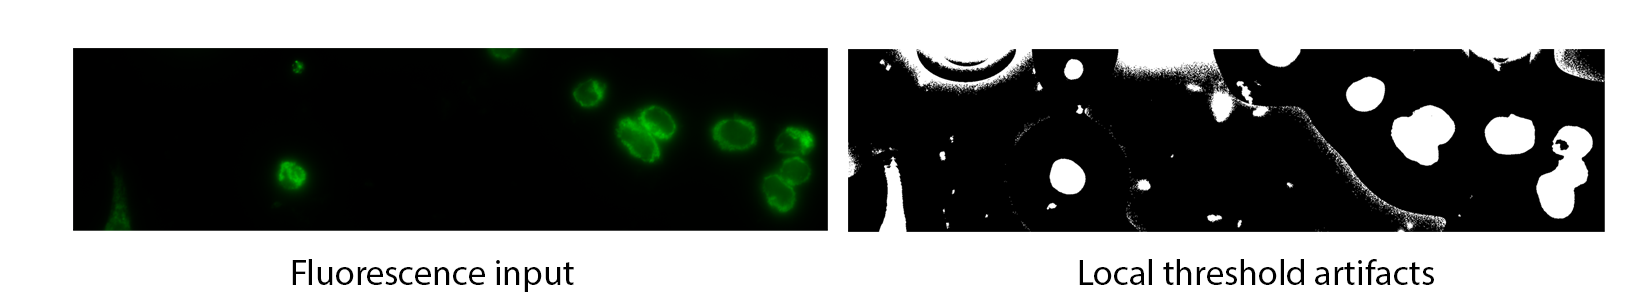
\includegraphics[width=\linewidth]{bilder/ER/artifacts.png}
		\caption{Artifacts from local thresholding algorithm}\label{fig:artifacts-er}
	\end{center}
\end{figure}
Such falsely recognized regions appeared in the nuclei as well, yet there they were easily filtered out based on the shape criteria. All nuclei are almost round and convex objects, whereas background artifacts are prolonged completely non-convex objects. Unfortunately, such filtration cannot be applied to ER imaging as very often ER from one cell is locate very close one to another one, and together they may form a long non-convex object as well. That is why it is very important to remove the background noise here first before applying a local threshold.

In order to do that one can first apply a rough "over-predictive" global thresholding, that will cover a true signal fully, including the "shine" around the ER, but will ignore the background noise. In the role of "over-predictove" global mean thresholding algorithm can be used (see Figure \ref{fig:er-segmentation-steps}.2). The mask created with the mean thresholding approach is used to zero out all the pixels that are not covered by it. And after that the local thresholding can be successfully applied with the \textit{block\_size} of $181$ (Figure \ref{fig:er-segmentation-steps}.4). Then  algorithm fills in all the holes in the middle of ER that might have appeared during the thresholding. Morphological opening (see Section TODO cite section) and Gaussian Blur with the squared kernel $3 \times 3$ are applied. Connected components are detected afterwards and filtered based on the limit of the area they occupy, this filters out mostly very small components from the mask which might be produced by the left out background noise. The whole algorithm overview is described below:

Segmentation steps are described in Algorithm \ref{alg:er-segmentation-steps} and also illustrated in Figure \ref{fig:er-segmentation-steps}.

\begin{algorithm}
    \caption{Fluorescence segmentation}
    \begin{algorithmic}
    \item 1. Normalize image
    \item 2. Apply global \textit{threshold\_mean} to receive initial mask.
    \item 3. Zero out pixels outside the mask
    \item 4. Apply local thresholding.  
    \item 5. Apply \textit{fill\_holes} transformation.
    \item 6. Morphological opening from OpenCV and Gaussian blur.
    \item 7. Run \textit{findContours} from OpenCV in order to obtain separate regions and filter out too small regions.
    \end{algorithmic}
    \label{alg:er-segmentation-steps}
\end{algorithm}    

\begin{figure}[htb]
    \begin{center}
        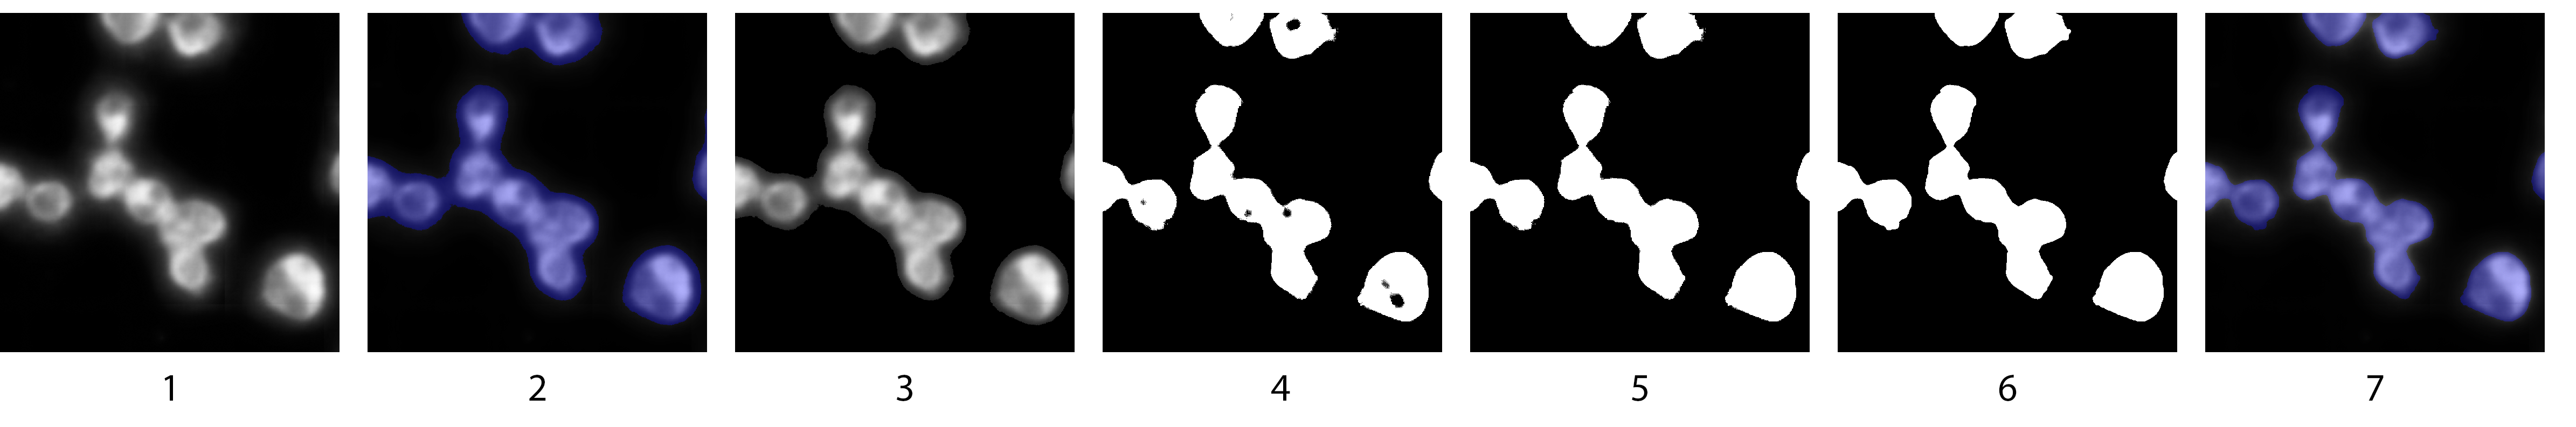
\includegraphics[width=0.3\linewidth]{bilder/ER/segmentation/segmentation.png}
        \caption{Segmentation steps in ER postprocessing}\label{fig:er-segmentation-steps}
    \end{center}
\end{figure}